\chapter{Założenia projektowe}
W rozdziale opisano główny problem oraz potencjalne ścieżki prowadzące do jego rozwiązania. Zamieszczono w nim również wynik przeprowadzonej analizy wymagań funkcjonalnych i niefunkcjonalnych dla mającej powstać aplikacji. Zaproponowano ponadto makiety interfejsu użytkownika oraz przedstawiono narzędzia i technologie wybrane do realizacji celu pracy.

% Описание проблемы:
% Существует проблема найти рабочую станцию зарядки, когда остается мало зарядки в автомобиле.
% Станция может не работать, плохо заряжать, может быть установлена так, что ей невозможно пользоваться, 
% различные сервисы, зачастую, ориентируются на конкретную фигрму заправок и могут не иметь самую актуальную информацию о появлении станций других производителей.
% Хочется просто взять телефон и прямо на карте увидеть где есть станции и посмотреть о ней отзывы реальных людей.

% В результате работы должно быть создано мобильное приложение в которм:
% Водители жлекторомобилей могут легко и быстро находить ближайшие зарядные станции и выбирать лучшую.
% Владельцы стнаций могут добавлять свои станции, что даст им дополнительную рекламу.
% Для определения качества станции должна использоваться система актуальных коментариев и оценок зарегестрированных пользователей.
% Каждый пользователь должен иметь собственный аккаунт для возможности пользоваться приложениемю
% Эта система позволит повысить качество зарядных пунктов.
% Это приложение полнстью поддеживается сообществом: создание и оценка станций производится пользователями.

% В пользовательском интерфейсе, которым я вляется мобильное приложение, должна быть интегрирована карта для упрощения поиска и создания мест.
% Должна быть реализована система регистарции и входа.
% Кроме пользовательского интерфейса долен быть реализована серверная часть, для обработки действий пользователей.
% А также база данных дляхранения станций и коментариев.

% Предположительный макет сервиса:
\section{Analiza biznesowa}
Podczas podróży pojazdami elektrycznymi sporym problemem jest znalezienie stacji ładowania, w której można byłoby doładować akumulatory. Znając nawet położenie takich stacji nie ma żadnej pewności, że stacje te aktualnie działają, że zapewniony jest do nich dostęp czy też posiadają odpowiednie oprzyrządowanie. Większość istniejących aplikacji mobilnych wspierających użytkowników w takich kwestiach najczęściej gromadzi dane dotyczące stacji konkretnych firm, bez żadnych wskazówek co do lokalizacji stacji ładowania konkurentów. Co więcej, nawet te dane, które są oferowane, bywają nieaktualne, nie mówiąc już o braku ocen wystawianych przez użytkowników. Problemy te można byłoby rozwiązać za pomocą aplikacji mobilnej. Wystarczyłoby, by aplikacja ta wyświetliła bieżącą pozycję użytkownika na mapie oraz pokazała stacje znajdujące się w pobliżu wraz z możliwością podglądu opinii na ich temat wystawionych przez innych użytkowników.

Aplikacja ta w szczególności mogłaby wspierać kierowców pojazdów elektrycznych w odnajdowaniu najbliższych stacji ładowania, pomagając w łatwy i przyjazny sposób wybrać stację najlepszą. Właściciele mogliby dostarczać informacji o swoich stacjach, co może robili by z chęcią z uwagi na ich dodatkową reklamę.

Aby stworzyć jakiś ranking stacji czy też obiektywnie oceniać ich jakość należałoby wprowadzić możliwość tworzenia aktualnych komentarzy wraz z wystawianiem oceny przez zarejestrowanych użytkowników. Każdy zarejestrowany użytkownik musiałby wtedy posiadać konto w systemie, by można było autoryzować jego działania.

Wdrożenie takiego systemu mogłoby przyczynić się do poprawy jakości usług świadczonych na stacjach ładowania pojazdów elektrycznych.
Jednak aby ten cel osiągnąć w pełni, potrzebne byłoby uzyskanie wsparcia od społeczności użytkowników.

\section{Zarys architektury systemu}
% TO DO: tutaj powinno być parę słów o architekturze - czyli komponentach, z jakich zbudowane ma być rozwiązania, jego otoczeniu, przepływie informacji
% Opis funkcji systemu powinien znaleźć się w analizie wymagań. Proszę odpowiednio przeredagować ten podrozdział
Interfejs użytkownika, którym jest aplikacja mobilna, musi mieć zintegrowaną mapę, aby ułatwić wyszukiwanie i tworzenie miejsc.
Należy wdrożyć system rejestracji i logowania. Oprócz interfejsu użytkownika musi być zaimplementowana część serwerowa do obsługi działań użytkowników.
A także baza danych do przechowywania stacji i komentarzy. Ten układ widać na rysunku \ref{fig:zarysuskladuserwisu}.
\begin{figure}[ht]
    \centering
        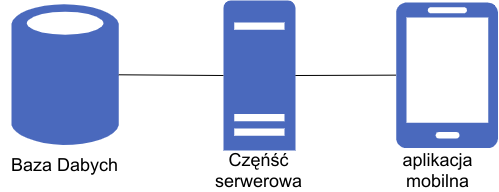
\includegraphics[width=0.4\linewidth]{rys02/uklad_wstepny.png}
        \caption{Zarys architektury budowanego rozwiązania \cite{diagrams_net}}
    \label{fig:zarysuskladuserwisu}
\end{figure}\newline

\section{Analiza wymagań}
\subsection{Wymagania funkcjonalne}
Wymagania funkcjonale definiują oczekiwany zakres funkcji dostarczanych przez tworzony system oraz jego zachowania. Wymagania te można definiować w języku naturalnym bądź też w języku formalnym. W niniejszej pracy wymagania przedstawiono na diagramie przypadków użycia (patrz rysunek~\ref{fig:usecasediagram}) oraz opisano tabelarycznie cel ich wdrożenia (patrz tabela~\ref{tab:wymaganiafunkcjonalne}).
Na diagramie przypadków użycia zwykle przedstawia się użytkowników w powiązaniu z dostępnymi dla nich funkcjami. W budowanej aplikacji istnieje tylko jeden typ użytkownika. 
% TO DO: Diagram do przerysowania (jest za wysoki - można przecież ułożyć przypadki logowania i rejestracji w poziomie, nie w pionie. Podobnie można poprzesuwać pozostałe przypadki. Owale są za duże w porównaniu do zawartego w nich tekstu. Niech nazwy przypadków będą pisane dużą literą
\begin{figure}[ht]
    \centering
        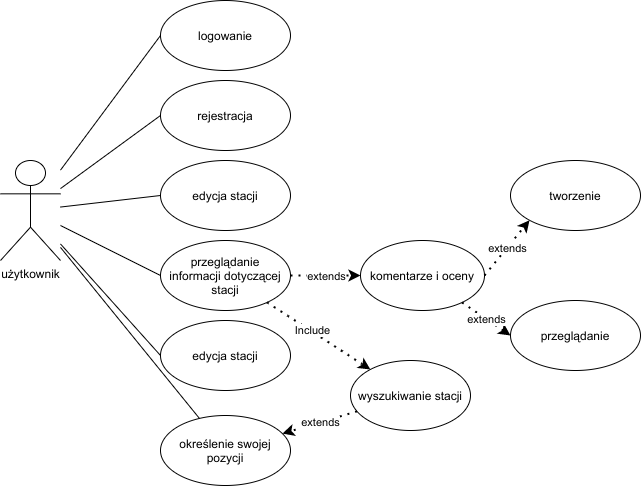
\includegraphics[width=0.7\linewidth]{rys02/use_case_diagram.png}
        \caption{dagram przypadków uzycia \cite{diagrams_net}}
    \label{fig:usecasediagram}
\end{figure}

% TO DO: Poprawić wpisy w tabeli: w pierwszej kolumnie powinny być te same nazwy przypadków do na diagramie, w drugiej - w miarę dokładny opis celu, jaki można osiągnąć (poprawione są tylko początkowe wiersze)
\begin{table}[htb] \small
    \caption{Wymagania funkcjonalne}
    \label{tab:wymaganiafunkcjonalne}
    \begin{tabularx}{\linewidth}{| r | p{6cm} | X |} 
    \hline
    № & Przypadek & Cel \\
    \hline
    1 & Logowanie & Pozwala użytkownikowi zalogować się do własnego konta \\ 
    \hline
    2 & Rejestracja & Pozwala na stworzenie konta (w bazie danych pojawia się nowy wpis) i otwiera możliwość zalogowania się. \\ 
    \hline
    3 & Użytkownik wyszykuje stacje ładowania obok wybranego miejsca  & Umożliwienie wyboru stacji dogodnej dla użytkownika \\
    \hline
    4 & Użytkownik ma możliwość określenia własnej pozycji & Wyszukiwanie stacji w sposób bardziej intuicyjny dla użytkownika  \\
    \hline
    5 & Użytkownik ma możliwość przyglądania mapy razem ze swoją lokalizacją oraz stacji ładowania obok wybranego miejsca & Ułatwienie wyszukiwania najwygodniejszej stacji ładowniczej \\
    \hline
    6 & Użytkownik ma możliwość wyszukiwania stacji ładowniczej według słów kluczowych & Wyszukiwanie dogodnej stacji z punktu widzenia typu lub nazwy stacji \\
    \hline
    7 & Użytkownik ma możliwość przeglądania informacji dotyczącej stacji, w tym oceny i komentarzy innych użytkowników & Podjęcie decyzji i dobór odpowiedniej dla użytkownika stacji \\
    \hline
    8 & Użytkownik ma możliwość wystawienia oceny i napisania komentarzy do wybranej stacji  & Określenie jakości stacji. Pozwala na aktualizację danuch dotyczących stacji ladowniczej \\
    \hline
    9 & Użytkownik ma możliwość dowdawania (oznaczenia, tworzenie) nowej stacji  & Aktualizacja informacji o dostępnych stacjach \\
    \hline
    10 & Użytkownik, który stworzył stację, ma możliwość zmiany informacji o tej stacji ładowniczej & Aktualizacja informacji istniejącej statji \\
    \hline
\end{tabularx}
\end{table}


\subsection{Wymagania niefunkcjonalne}
W tabeli \ref{tab:wymaganianiefunkcjonalne} przdstawione wymagania niefunkcjonalne: krótki opis wymagania, typ (jakiej dziedziny to dotyczy) oraz uwagi do tego wymagania.
\begin{table}[htb] \small
    \caption{Wymagania niefunkcjonalne}
    \label{tab:wymaganianiefunkcjonalne}
    \begin{tabular}{| m{0.5cm} | m{3cm} | m{5.75cm} | m{5.75cm} |} 
    \hline
    № & typ & Opis & Uwagi \\
    \hline
    1 & Bezpiczeństwo & Hasła muszą być przechowywane w biezpicznej formie & Hasła nie przchowyją się w pierwotnej formie, tylko w formie zaszyfrowanej \\ 
    \hline
    2 & Bezpiczeństwo & Małe ryzyka przechwytywania hasła przez trzecich osób podczas komunikacji interfejsu użytkownika i części serwerowej & Autentykacja użytkownika na serwerze powinna zachodzić za pomocą tokenów \\ 
    \hline
    3 & Przenoszlność & wdrożenie systemu powinno być szybkie i łatwe & \\ 
    \hline
    4 & Konfigurowalność & Zmiana ustaleń bez konieczosści rekompilacji części serwerowej & Zarządzaniem portu na którym działa część serwerowa, wymiana adresu oraz nazwy kolekcji bazy danuch, musi być możliwa za pomocą pliku konfiguracyjnego \\ 
    \hline
    5 & Estetyczne & Przyjazny interfajs użytkownika & Intuicyjny i zrozumiały interfejs \\ 
    \hline
    6 & Ergonomia & Interfejs w języku angielskim & Możliwość kożystania z aplikacji przez dużą libzi \\
    \hline
    7 & Przenoszlność & Aplikacja mobilna musi działać na 90\% lub więcej telefonów pracujących na systemie Android & Możliwość kożystania z aplikacji przez dużą ilość ludzi \\
    \hline
    8 & Estetyczne & kolory muszą być odpowiednio dopasowane & Wykorzystanie małej dopasowanych do sobie ilośći kolorów  \\
    \hline
    9 & Wydajność & Srzybka reakcja systemu & System musi szybko reagować na działania użytkownika \\
    \hline
    10 & Informatywność & System powinien powiadomiać o błędach i sukcesach  & Podczas rażądzania systemem użytkownik powinin zawze wiedzieć jaki wynik jego działania \\
    \hline
    11 & Ergonomia & Wykorzystanie z aplikacji mobilnej za pomocą jednej ręki & Przyciski muszą znajdować się w dolnej części ekranu lub znajdować się w dostępnym miejscu \\
    \hline
    12 & Estetyczne & Wszystkie elementy muszą być w jednym stylu & Niedopuszczalne jest użycie różnych czcionek oraz ciągłej zmiany kolorów \\
    \hline
    13 & Dostęp & Część serwerowa zrobiona zgodnie z regułami Rest (ang.~\emph{Representational State Transfer}) API (ang.~\emph{Application Programming Interface}) & Przestrzeganie się Best Prakties Rest API \cite{rest_api_best}] \\
    \hline
    14 & Ergonomia & Dla realizacji mapy wykorzystuję się Google Maps[index] & Ułatwia rozumienie interfejsu dla użytkowników \\
    \hline
\end{tabular}
\end{table}
\newpage
\subsection{Narzędzia i technologie}
Do stworzenia aplikacji mobilnej, części serwerowej oraz bazy danych wybrano następujące narzędzia i technologie:
\begin{multicols}{3}
\begin{itemize}
    \item Visual Studio Code;
    \item Go;
    \item REST API;
    \item JWT;
    \item MongoDB;
    \item Redis;
    \item Android Studio;
    \item Gradle;
    \item Android SDK;
    \item Java JDK 8;
    \item RxJava 2;
    \item Google Cloud Platform;
    \item GMS;
    \item Docker;
\end{itemize}
\end{multicols}


\noindent\textbf{Visual Studio Code} -- to darmowy edytor kodu źródłowego wyprodukowany przez firmę Microsoft. Działa na systemach Windows, Linux, macOS. Wspiera on różne języki programowania oraz posiada możliwość rozszerzeń dzięki mechanizmowi plug-inów. Wśród jego funkcji można wymienić: podświetlanie składni, IntelliSense, refaktoryzacja, debugowanie i inne.~\cite{vscode} \\

\noindent\textbf{Go} (golang) -- jest językiem programowania stworzonym przez firmę Google. Pozwala tworzyć aplikacje wielowątkowe kompilowane dla systemów Linux, Windows, macOS, FreeBSD, Android i innych. Język jest przeznaczony do budowania serwisów działających efektywnie pod wysokim obciążeniem w środowisku rozproszonym i z wielowątkowymi procesorami.~\cite{golang1,golang2,golang3,godoc} \\

\noindent\textbf{REST API} (ang.~\emph{Representational State Transfer Application Programming Interface}) -- jest podejściem stosowanym w tworzenia interfejsów programistycznych aplikacji webowych. Obowiązują w nim następujące zasady: komunikacja w architekturze klient-serwer (serwer nasłuchuje na żądania wysyłane przez klienta oraz udziela na nie odpowiedzi), brak stanu (serwer nie przechowuje stanu klienta, wszystkie potrzebne informacje są wysyłane wraz z żądaniem), buforowanie (buforowanie danych jest dozwolone, jeśli w odpowiedzi jest na to zgoda), jednorodność interfejsu (ograniczenia stylu pisania), wielopoziomowość systemu (komponenty systemu mają bezpośredni dostęp tylko do sąsiednich warstw), łatwość rozszerzenia funkcjonalności (opcjonalnie).  \cite{rest_api,rest_api_best} \\

\noindent\textbf{JWT} (ang.~\emph{JSON Web Token}) -- jest standardem wykorzystywanym do tworzenia tokenów dostępu. Za pomocą JWT sprawdza się, czy wchodzące dane zostały wysłane przez autoryzowane źródło. Wykorzystywany model informacyjny składa się z trzech części: nagłówka (informacja o tym, w jaki sposób odszyfrować token), danych (zaszyfrowane dane) oraz sygnatury. Każdy token ma określony okres ważności. Nie może być oznaczony jako nieważny, dopóki ten okres się nie zakończy.~\cite{jwt} \\

\noindent\textbf{MongoDB} -- jest dokumentową bazą danych zaliczaną do rozwiązań typu NoSQL (ang.~\emph{Not only Structured Query Language}). Formatem przechowywania danych jest BSON (ang.~\emph{Binary JavaScript Object Notation}). Działa na licencji SSPL (ang.~\emph{Server Side Public License}). Wykorzystuje technikę segmentacji obiektów bazy danych, co pozwala na bilansowanie obciążenia.~\cite{mongoDB,mongoDB_doc,mongodb_habr} \\

\noindent\textbf{Redis} -- to system zarządzania bazami danych zaliczany do rozwiązań typu NoSQL, operujący na strukturach typu ,,klucz-wartość''. 
Najczęściej używa się go do implementacji baz danych w pamięci podręcznej, głównie brokerów wiadomości.~\cite{redis} \\

\noindent\textbf{Android Studio} -- to zintegrowane środowisko programistyczne stworzone przez firmę JetBrains na podstawie IntelliJ IDEA, służące do budowania aplikacji na platformie Android. Środowisko to jest dostępne do systemów Windows, Linux, macOS na bezpłatnej licencji Apache 2.0.~\cite{android_doc,android_studio} \\

\noindent\textbf{Gradle} -- jest systemem automatycznego budowania aplikacji oraz zarządzania zależnościami w aplikacjach rozwijanych w języku Java.~\cite{gradle,gradle_android_doc} \\

\noindent\textbf{Android SDK} -- jest pakietem narzędzi dostarczonym przez firmę Google. Służy do tworzenia aplikacji mobilnych działających pod kontrolą systemu Android. W skład SDK (ang.~\emph{Software Development Kit}) wchodzą: zestaw bibliotek Android i Java, emulator telefonu, debugger, dokumentacja, szablony prostych aplikacji.~\cite{android_studio} \\

\noindent\textbf{Java JDK 8} -- jest zestawem narzędzi programistycznych stosowanym do tworzenia oprogramowania na platformie Java. JDK (ang.~\emph{Java Development Kit}) zawiera: kompilator języka Java, przykłady, dokumentację, środowisko uruchomieniowe JRE (ang.~\emph{Java Runtime Environment}).
Java jest obiektowym językiem ogólnego zastosowania, kompilowanym do niezależnego od systemu operacyjnego kodu bajtowego uruchamianego na maszynie wirtualnej. Powstał w firmie Sun Microsystems, którą przejęła firma Oracle.~\cite{java_doc} 
Do budowy aplikacji wykorzystano JDK w wersji 1.8 (nie jest to najnowsza wersja, ale z uwagi na duże wsparcie i liczne zastosowania pozostaje wciąż popularna). \\

\noindent\textbf{RxJava 2} -- jest biblioteką pozwalającą na stosowanie reaktywnego programowania w języku Java. Programowanie reaktywne jest paradygmatem programowania pozwalającym na posługiwanie się asynchronicznymi strumieniami danych (sekwencjami zdarzeń uporządkowanymi według czasu).
Biblioteka ta przydaje się do zapewnienia ciągłości funkcjonowania interfejsu użytkownika nawet w podczas realizacji złożonej logiki obliczeniowej, na przykład podczas oczekiwania na odpowiedzi serwera. \\

\noindent\textbf{Google Cloud} -- jest pakietem usług udostępnianych w chmurze Google. Do tego pakietu należą znane usługi, jak: Google Search, Gmail, Google Drive, Youtube. Ponadto w ramach tego pakietu możliwe są obliczenie i przechowywanie danych, uczenie maszynowe i inne usługi, które Google wykorzystuje w swoich projektach. \cite{google_cloud} 
Usługa ta jest odpłatna, a wysokość opłat zależy od wybranego planu biznesowego oraz stopnia wykorzystania chmury. Jeśli koszty użycia serwisów kształtują się na poziomie niższym niż 200 dolarów miesięcznie, wtedy opłaty nie są egzekwowane przez Google. W tej pracy inżynierskiej wykorzystano serwis Static Maps \cite{google_cloud_pricing}. Jest on darmowy przy tworzeniu oprogramowania do telefonów z wykorzystaniem Android Maps SDK for Android \cite{maps_sdk}. \\

\noindent\textbf{GMS} (ang.~\emph{Google Mobile Services}) -- to zestaw najpopularniejszych aplikacji i API, jak  Goole Maps, Google Paly Store, Gmail Google Drive Google Duo, Google Chrome, Google Photos, Google TV, Youtube, Youtube Music adresowanych przez Google na urządzenia mobilne. \\

\noindent\textbf{Docker} -- jest oprogramowaniem przeznaczonym do automatyzacji wdrażania i zarządzania aplikacjami. Aplikacje uruchamiają się w kontenerach. Docker pozwala na upakowanie aplikacji oraz wszystkich zależności w niezależny od podstawowego systemu kontener, który może być łatwo przeniesiony na dowolny *nix system.~\cite{docker,docker_doc} \\

% Jako Baza danych wykorzystuje się NoSQL (ang. (ang.~\emph{Not only Structured Query Language}) baza danych MongoDB \cite{mongoDB,mongoDB_doc}.
% Część serwerowa napisana w języku Go \cite{golang1,golang2,golang3,godoc} w architekturze Rest API \cite{rest_api_best}.
% Część serwerowa i Baza Danych muszą uruchamiać się w Docker kontenerze \cite{docker,docker_doc}.
% Aplikacja mobilna działa w systemie Android za pomocą Android Studio \cite{android_doc,android_studio,gradle,gradle_android_doc} w języku Java \cite{java_doc}.
% Dla realizacji Google Maps w aplikacji mobilnej wykorzystuję się serwis Google Cloud \cite{google_cloud} Maps SDK for Android (ang.~\emph{Maps Software development kit for Android}) \cite{maps_sdk}.
% 
\subsection{Makiety interfejsu użytkownika}
Po analizie wymagań zostały stworzone możliwe makiety aplikacji, która ma powstać.

Na dole ekranu aplikacji znajduje się główne menu zawierające 4 pozycje: mapę, wyszukiwanie stacji, tworzenie stacji i parametry.
Na rysunku \ref{fig:search_makiet}a przedstawiono pierwszy etap wyszukiwania stacji ładowania.
Pod polem wyszukiwania znajduje się rozwijane menu, które pozwala wybierać typ wyszukiwania, w tym wyszukiwanie na podstawie pozycji użytkownika oraz nazwy i opisu stacji.
Poniżej znajduje się możliwość do zmiany dystansu wyszukiwania oraz przycisk wyszukiwania.
\begin{figure}[ht]
	\centering
  \begin{tabular}{@{}rl@{\hspace{10mm}}rl@{}}
  a) & \vtop{\vskip-2ex\hbox{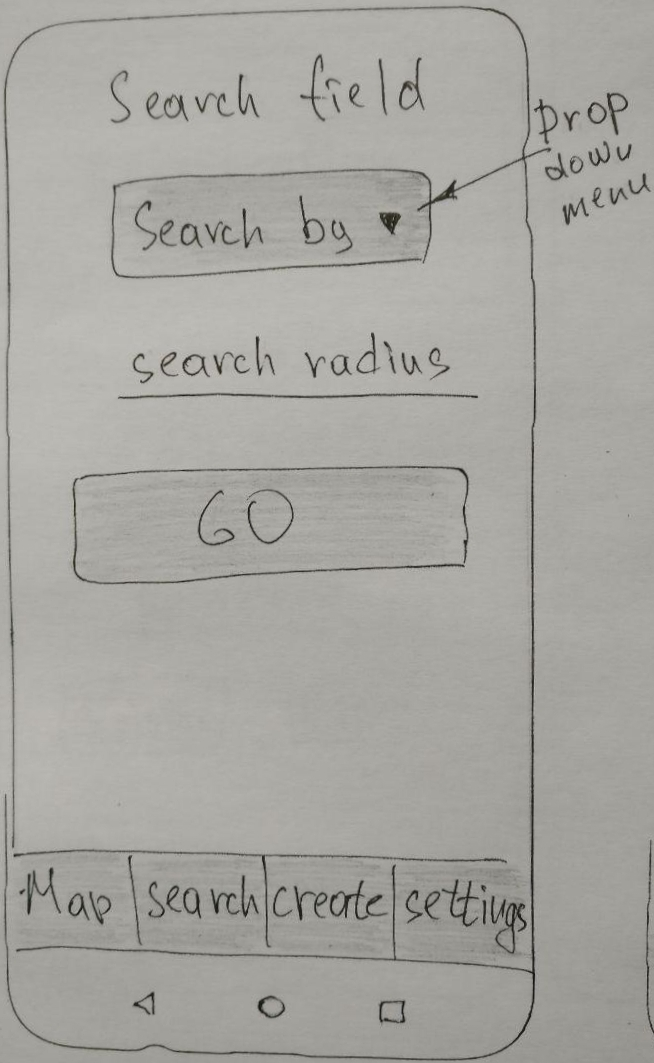
\includegraphics[width=0.30\linewidth]{rys02/search_makiet.jpg}}} &
	b) & \vtop{\vskip-2ex\hbox{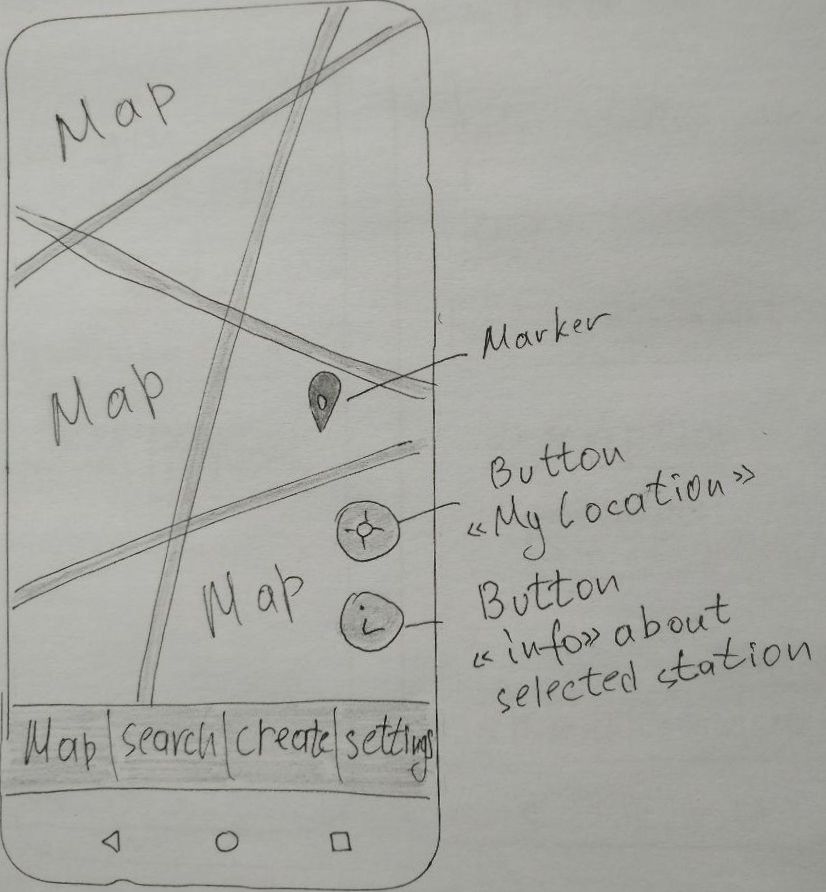
\includegraphics[width=0.45\linewidth]{rys02/main_makiet.jpg}}} 
		\end{tabular}
        \caption{Makiety interfejsów aplikacji mobilnej: a) strona wyszukiwania stacji ładowania, b) strona główna.}
    \label{fig:search_makiet}
\end{figure}

Na rysunku~\ref{fig:search_makiet}b przedstawiono makietę pozwalającą dokonać wyboru stacji ładowania. Stacje poznaczone znacznikami na mapie. Dla otrzymania informacji o wybranej stacji (wybierany jest markier na mapie) oraz wyświetlania pozycji użytkownika wykorzystują się okrągłe przyciski z lewej strony ekranu.

Podczas tworzenia stacji ładowania  dla wygody użytkowania można wybrać miejsce na mapie poprzez odpowiedni przycisk (rys.~\ref{fig:create_makiet}a).
% TO DO: proszę ułożyć dwie makiety obok siebie, jak w przykładzie powyżej
% DONE:
\begin{figure}[ht]
	\centering
    \begin{tabular}{@{}rl@{\hspace{10mm}}rl@{}}
        a) & \vtop{\vskip-2ex\hbox{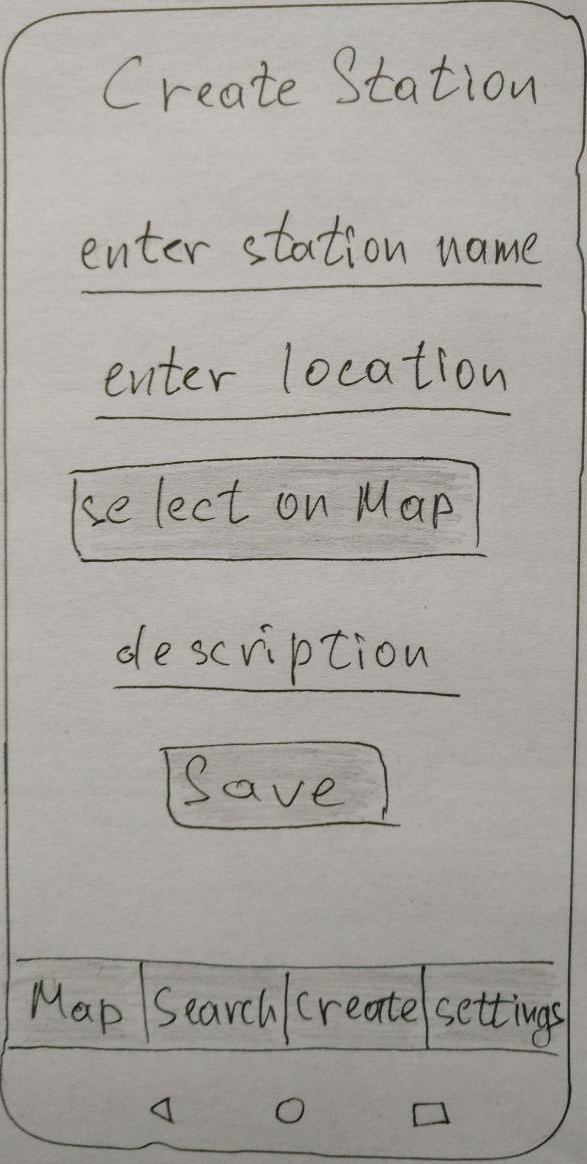
\includegraphics[width=0.30\linewidth]{rys02/create_makiet.jpg}}} &
        b) & \vtop{\vskip-2ex\hbox{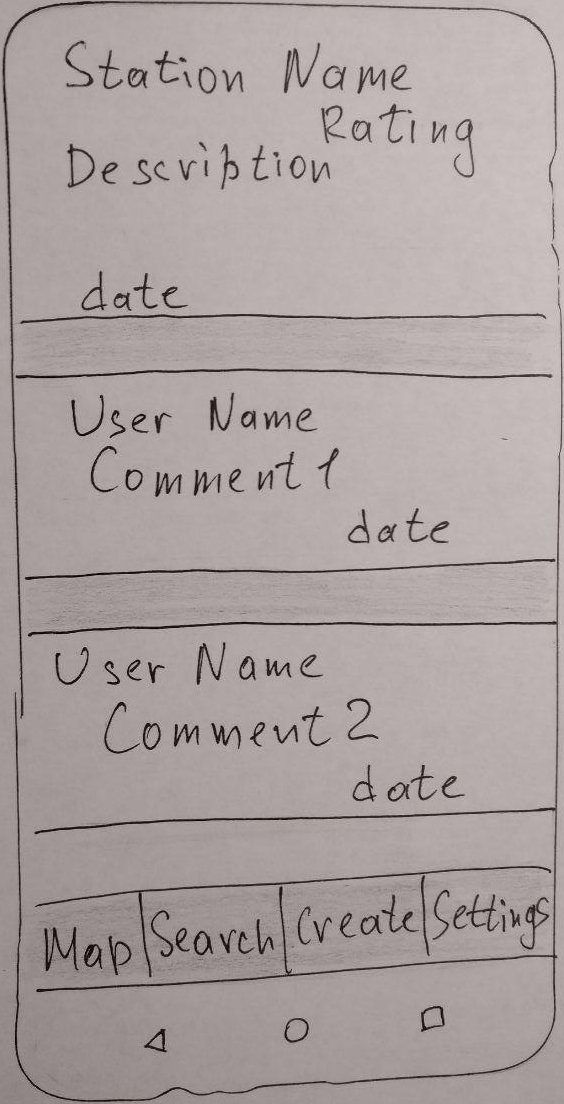
\includegraphics[width=0.30\linewidth]{rys02/station_makiet.jpg}}} 
    \end{tabular}
    \caption{Makiety interfejsów aplikacji mobilnej: a) strona tworzenia stacji ładowania, b) strona informacji o stacji ładowania.}
    \label{fig:create_makiet}
\end{figure}

Na stronie informacji o stacji oprócz nazwy stacji, opisu oraz oceny, wyliczonej na podstawie komentarzy oceny, znajdują się komentarzy użytkowników uporządkowane od najnowszego (rys.\ref{fig:create_makiet}b) .

Do rejestracji i logowania wykorzystują się dwa różne ekrany pokazane, odpowiednio, na rysunku~\ref{fig:login_makiet}a oraz rysunku~\ref{fig:login_makiet}b)
\begin{figure}[ht]
	\centering
  \begin{tabular}{@{}rl@{\hspace{10mm}}rl@{}}
  a) & \vtop{\vskip-2ex\hbox{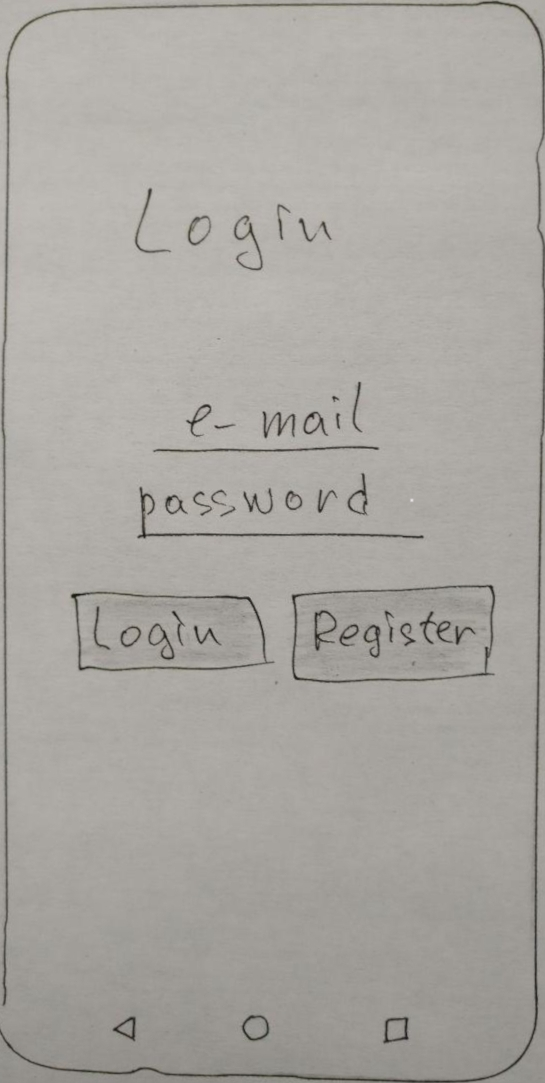
\includegraphics[width=0.30\linewidth]{rys02/login_makiet.jpg}}} &
	b) & \vtop{\vskip-2ex\hbox{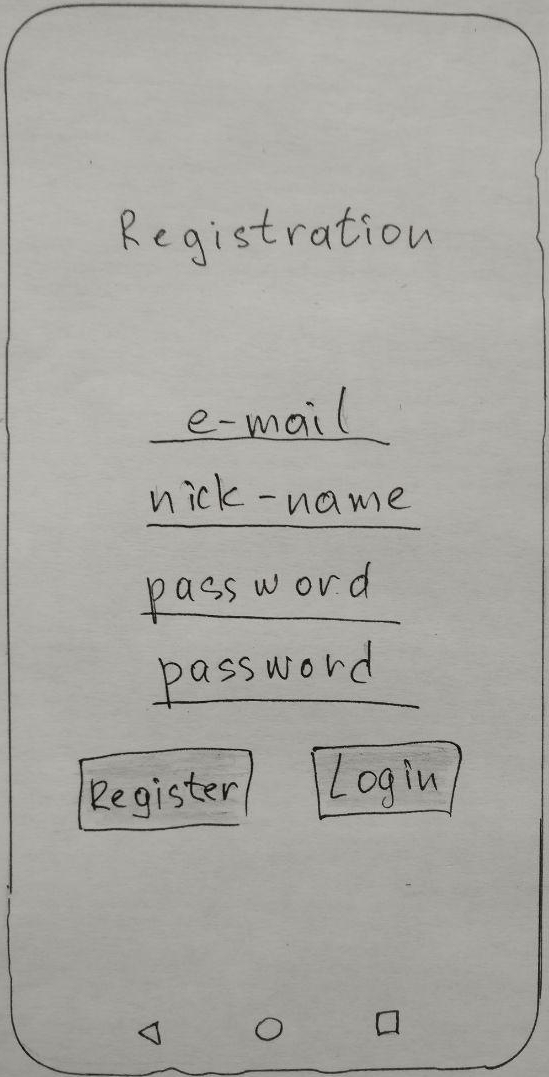
\includegraphics[width=0.30\linewidth]{rys02/register_makiet.jpg}}} 
		\end{tabular}
        \caption{Makiety interfejsów aplikacji mobilnej: a) strona logowania, b) strona rejestracji.}
    \label{fig:login_makiet}
\end{figure}


% \paragraph{Część serwerowa:}
% \begin{itemize}
%     \item Visual Studio Code
%     \item Go
%     \item MongoDB
%     \item Redis
%     \item Docker ?
%     \item Docker-compose ?
%     \item Go Modules
%     \item gorilla/mux
%     \item sirupsen/logrus
%     \item mongo-driver
%     \item go-redis/redis
%     \item go-ozzo/ozzo-validation
%     \item yaml.v2
%     \item google/uuid
% \end{itemize}

% \paragraph{Aplikacja mobilna:}
% \begin{itemize}
%     \item Android Studio
%     \item Java   
%     \item ? gradle ?
%     \item RxJava
%     \item OkHttp 3
%     \item Retrofit 2
%     \item Maps SDK for Android
%     \item Google Play services APIs
%     \item gson
% \end{itemize}

% \paragraph{Testowanie: ??}
% \begin{itemize}
%     \item Postman
%     \item MongoDB Compass
%     \item stretchr/testify ??
% \end{itemize}


% \paragraph{Paragraf}
% Tekst\newline
% Tekst
